\documentclass{whiteboard}
\begin{document}
\begin{frame}[plain,t]
 \bbcover{Grafos}{Representação de grafos}{Prof. Edson Alves}{Faculdade UnB Gama}
\end{frame}

\begin{frame}[plain,t]
\begin{tikzpicture}
\node[draw,opacity=0] at (0, 0) {x};
\node[draw,opacity=0] at (14, 8) {x};
 \node[anchor=west] at (0, 6) { \Large \bbbold{Matriz de adjacências} };
\end{tikzpicture}
\end{frame}

\begin{frame}[plain,t]
\begin{tikzpicture}
\node[draw,opacity=0] at (0, 0) {x};
\node[draw,opacity=0] at (14, 8) {x};
 \node[anchor=west] at (0, 6) { \Large \bbbold{Matriz de adjacências} };
 \node[anchor=west] at (1, 5) { $\star$ \bbtext{Seja $G$ um grafo com $N$ vértices } };
\end{tikzpicture}
\end{frame}

\begin{frame}[plain,t]
\begin{tikzpicture}
\node[draw,opacity=0] at (0, 0) {x};
\node[draw,opacity=0] at (14, 8) {x};
 \node[anchor=west] at (0, 6) { \Large \bbbold{Matriz de adjacências} };
 \node[anchor=west] at (1, 5) { $\star$ \bbtext{Seja $G$ um grafo com $N$ vértices } };
 \node[anchor=west] at (1, 4) { $\star$ \bbtext{Assuma que cada vértice seja associado a um inteiro  positivo em $[1, N]$} };
\end{tikzpicture}
\end{frame}

\begin{frame}[plain,t]
\begin{tikzpicture}
\node[draw,opacity=0] at (0, 0) {x};
\node[draw,opacity=0] at (14, 8) {x};
 \node[anchor=west] at (0, 6) { \Large \bbbold{Matriz de adjacências} };
 \node[anchor=west] at (1, 5) { $\star$ \bbtext{Seja $G$ um grafo com $N$ vértices } };
 \node[anchor=west] at (1, 4) { $\star$ \bbtext{Assuma que cada vértice seja associado a um inteiro  positivo em $[1, N]$} };
 \node[anchor=west] at (1, 3) { $\star$ \bbtext{Na matrix de adjacências $A_{N\times N}$ o elemento $a_{ij}$ é o peso da aresta $(i, j)$} };
\end{tikzpicture}
\end{frame}

\begin{frame}[plain,t]
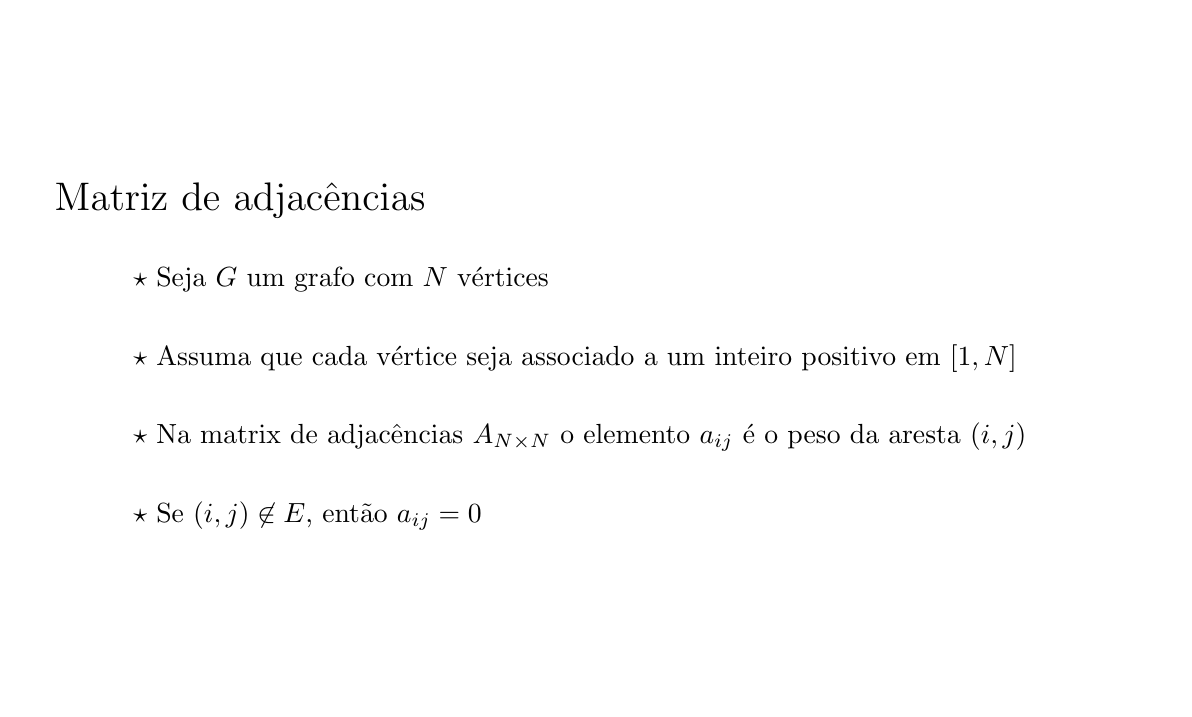
\begin{tikzpicture}
\node[draw,opacity=0] at (0, 0) {x};
\node[draw,opacity=0] at (14, 8) {x};
 \node[anchor=west] at (0, 6) { \Large \bbbold{Matriz de adjacências} };
 \node[anchor=west] at (1, 5) { $\star$ \bbtext{Seja $G$ um grafo com $N$ vértices } };
 \node[anchor=west] at (1, 4) { $\star$ \bbtext{Assuma que cada vértice seja associado a um inteiro  positivo em $[1, N]$} };
 \node[anchor=west] at (1, 3) { $\star$ \bbtext{Na matrix de adjacências $A_{N\times N}$ o elemento $a_{ij}$ é o peso da aresta $(i, j)$} };
 \node[anchor=west] at (1, 2) { $\star$ \bbtext{Se $(i, j)\not\in E$, então $a_{ij} = 0$} };
\end{tikzpicture}
\end{frame}

\begin{frame}[plain,t]
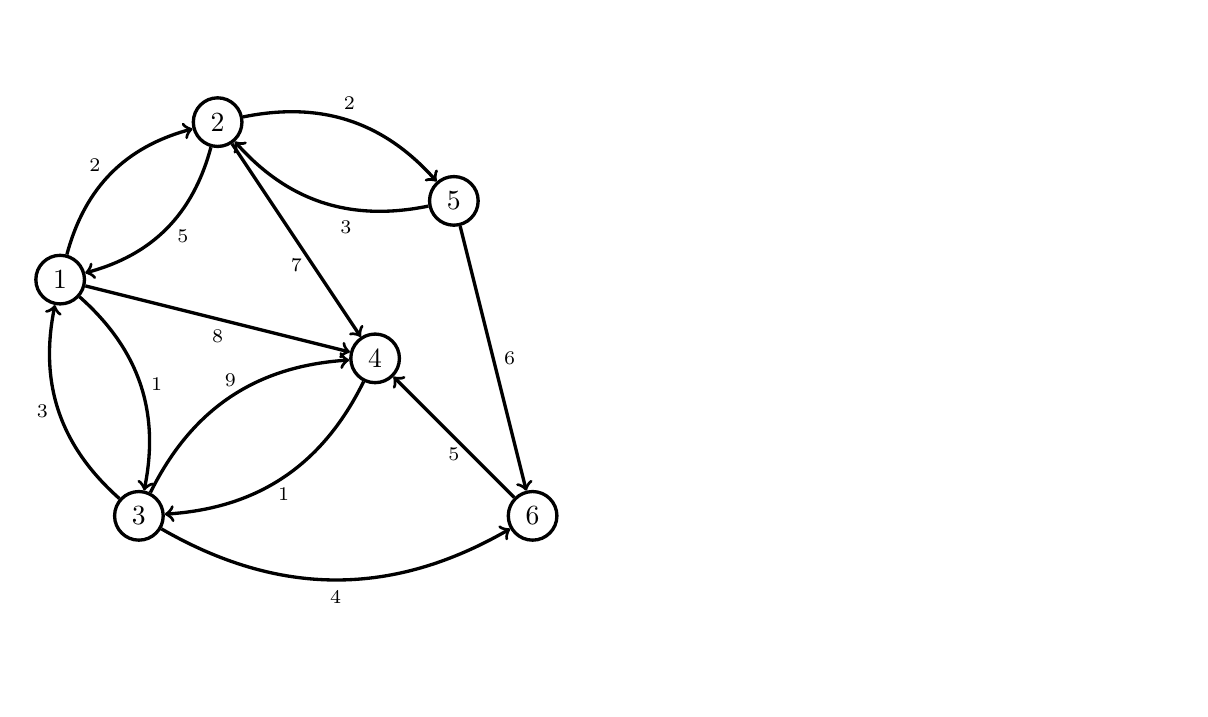
\begin{tikzpicture}
\node[draw,opacity=0] at (0, 0) {x};
\node[draw,opacity=0] at (14, 8) {x};
 \node[draw,circle,very thick] (A) at (0, 5) { \bbtext{1} };
 \node[draw,circle,very thick] (B) at (2, 7) { \bbtext{2} };
 \node[draw,circle,very thick] (C) at (1, 2) { \bbtext{3} };
 \node[draw,circle,very thick] (D) at (4, 4) { \bbtext{4} };
 \node[draw,circle,very thick] (E) at (5, 6) { \bbtext{5} };
 \node[draw,circle,very thick] (F) at (6, 2) { \bbtext{6} };
 \draw[->,very thick] (A) to [bend left] node[anchor=east,yshift=0.1cm] { \scriptsize $\bbinfo{2}$ } (B);
 \draw[->,very thick] (B) to [bend left] node[anchor=west,yshift=-0.1cm] { \scriptsize $\bbinfo{5}$ } (A);
 \draw[->,very thick] (A) to [bend left] node[anchor=west] { \scriptsize $\bbinfo{1}$ } (C);
 \draw[->,very thick] (C) to [bend left] node[anchor=east] { \scriptsize $\bbinfo{3}$ } (A);
 \draw[->,very thick] (D) to [bend left] node[anchor=north] { \scriptsize $\bbinfo{1}$ } (C);
 \draw[->,very thick] (C) to [bend left] node[anchor=south] { \scriptsize $\bbinfo{9}$ } (D);
 \draw[->,very thick] (B) to [bend left] node[anchor=south] { \scriptsize $\bbinfo{2}$ } (E);
 \draw[->,very thick] (E) to [bend left] node[anchor=north,xshift=0.3cm,yshift=-0.1cm] { \scriptsize $\bbinfo{3}$ } (B);
 \draw[->,very thick] (A) -- node[anchor=north] { \scriptsize $\bbinfo{8}$ } (D);
 \draw[->,very thick] (B) -- node[anchor=north,yshift=-0.1cm] { \scriptsize $\bbinfo{7}$ } (D);
 \draw[->,very thick] (C) to [bend right] node[anchor=north] { \scriptsize $\bbinfo{4}$ } (F);
 \draw[->,very thick] (F) -- node[anchor=north] { \scriptsize $\bbinfo{5}$ } (D);
 \draw[->,very thick] (E) -- node[anchor=west] { \scriptsize $\bbinfo{6}$ } (F);
\end{tikzpicture}
\end{frame}

\begin{frame}[plain,t]
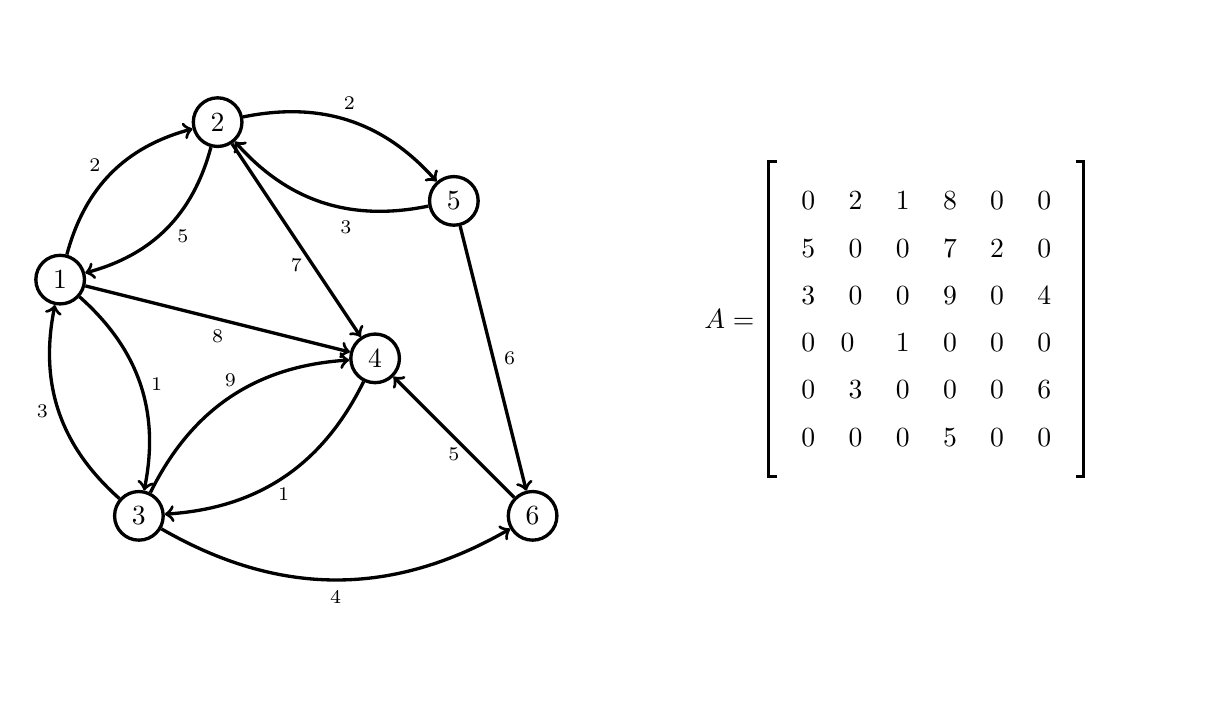
\begin{tikzpicture}
\node[draw,opacity=0] at (0, 0) {x};
\node[draw,opacity=0] at (14, 8) {x};
 \node[draw,circle,very thick] (A) at (0, 5) { \bbtext{1} };
 \node[draw,circle,very thick] (B) at (2, 7) { \bbtext{2} };
 \node[draw,circle,very thick] (C) at (1, 2) { \bbtext{3} };
 \node[draw,circle,very thick] (D) at (4, 4) { \bbtext{4} };
 \node[draw,circle,very thick] (E) at (5, 6) { \bbtext{5} };
 \node[draw,circle,very thick] (F) at (6, 2) { \bbtext{6} };
 \draw[->,very thick] (A) to [bend left] node[anchor=east,yshift=0.1cm] { \scriptsize $\bbinfo{2}$ } (B);
 \draw[->,very thick] (B) to [bend left] node[anchor=west,yshift=-0.1cm] { \scriptsize $\bbinfo{5}$ } (A);
 \draw[->,very thick] (A) to [bend left] node[anchor=west] { \scriptsize $\bbinfo{1}$ } (C);
 \draw[->,very thick] (C) to [bend left] node[anchor=east] { \scriptsize $\bbinfo{3}$ } (A);
 \draw[->,very thick] (D) to [bend left] node[anchor=north] { \scriptsize $\bbinfo{1}$ } (C);
 \draw[->,very thick] (C) to [bend left] node[anchor=south] { \scriptsize $\bbinfo{9}$ } (D);
 \draw[->,very thick] (B) to [bend left] node[anchor=south] { \scriptsize $\bbinfo{2}$ } (E);
 \draw[->,very thick] (E) to [bend left] node[anchor=north,xshift=0.3cm,yshift=-0.1cm] { \scriptsize $\bbinfo{3}$ } (B);
 \draw[->,very thick] (A) -- node[anchor=north] { \scriptsize $\bbinfo{8}$ } (D);
 \draw[->,very thick] (B) -- node[anchor=north,yshift=-0.1cm] { \scriptsize $\bbinfo{7}$ } (D);
 \draw[->,very thick] (C) to [bend right] node[anchor=north] { \scriptsize $\bbinfo{4}$ } (F);
 \draw[->,very thick] (F) -- node[anchor=north] { \scriptsize $\bbinfo{5}$ } (D);
 \draw[->,very thick] (E) -- node[anchor=west] { \scriptsize $\bbinfo{6}$ } (F);
 \node at (8.5, 4.5) { $A = $ };
 \draw[very thick] (9.1, 6.5) -- (9, 6.5) -- (9, 2.5) -- (9.1, 2.5);
 \draw[very thick] (12.9, 6.5) -- (13, 6.5) -- (13, 2.5) -- (12.9, 2.5);
 \node at (9.5, 6) { \bbinfo{0} };
 \node at (10.1, 6) { \bbinfo{2} };
 \node at (10.7, 6) { \bbinfo{1} };
 \node at (11.3, 6) { \bbinfo{8} };
 \node at (11.9, 6) { \bbinfo{0} };
 \node at (12.5, 6) { \bbinfo{0} };
 \node at (9.5, 5.4) { \bbinfo{5} };
 \node at (10.1, 5.4) { \bbinfo{0} };
 \node at (10.7, 5.4) { \bbinfo{0} };
 \node at (11.3, 5.4) { \bbinfo{7} };
 \node at (11.9, 5.4) { \bbinfo{2} };
 \node at (12.5, 5.4) { \bbinfo{0} };
 \node at (9.5, 4.8) { \bbinfo{3} };
 \node at (10.1, 4.8) { \bbinfo{0} };
 \node at (10.7, 4.8) { \bbinfo{0} };
 \node at (11.3, 4.8) { \bbinfo{9} };
 \node at (11.9, 4.8) { \bbinfo{0} };
 \node at (12.5, 4.8) { \bbinfo{4} };
 \node at (9.5, 4.2) { \bbinfo{0} };
 \node at (10, 4.2) { \bbinfo{0} };
 \node at (10.7, 4.2) { \bbinfo{1} };
 \node at (11.3, 4.2) { \bbinfo{0} };
 \node at (11.9, 4.2) { \bbinfo{0} };
 \node at (12.5, 4.2) { \bbinfo{0} };
 \node at (9.5, 3.6) { \bbinfo{0} };
 \node at (10.1, 3.6) { \bbinfo{3} };
 \node at (10.7, 3.6) { \bbinfo{0} };
 \node at (11.3, 3.6) { \bbinfo{0} };
 \node at (11.9, 3.6) { \bbinfo{0} };
 \node at (12.5, 3.6) { \bbinfo{6} };
 \node at (9.5, 3.0) { \bbinfo{0} };
 \node at (10.1, 3.0) { \bbinfo{0} };
 \node at (10.7, 3.0) { \bbinfo{0} };
 \node at (11.3, 3.0) { \bbinfo{5} };
 \node at (11.9, 3.0) { \bbinfo{0} };
 \node at (12.5, 3.0) { \bbinfo{0} };
\end{tikzpicture}
\end{frame}

\begin{frame}[plain,t]
\begin{tikzpicture}
\node[draw,opacity=0] at (0, 0) {x};
\node[draw,opacity=0] at (14, 8) {x};
 \node[anchor=west] at (0, 7) { \Large \bbbold{Características das matrizes de adjacências} };
\end{tikzpicture}
\end{frame}

\begin{frame}[plain,t]
\begin{tikzpicture}
\node[draw,opacity=0] at (0, 0) {x};
\node[draw,opacity=0] at (14, 8) {x};
 \node[anchor=west] at (0, 7) { \Large \bbbold{Características das matrizes de adjacências} };
 \node[anchor=west] at (1, 6) { $\star$ \bbtext{Se $G$ é não poderado, $a_{ij} \in [0, 1]$ } };
\end{tikzpicture}
\end{frame}

\begin{frame}[plain,t]
\begin{tikzpicture}
\node[draw,opacity=0] at (0, 0) {x};
\node[draw,opacity=0] at (14, 8) {x};
 \node[anchor=west] at (0, 7) { \Large \bbbold{Características das matrizes de adjacências} };
 \node[anchor=west] at (1, 6) { $\star$ \bbtext{Se $G$ é não poderado, $a_{ij} \in [0, 1]$ } };
 \node[anchor=west] at (1, 5) { $\star$ \bbtext{Se $G$ é multigrafo, $a_{ij}$ pode registrar o número de ocorrências de $(i, j)$ } };
\end{tikzpicture}
\end{frame}

\begin{frame}[plain,t]
\begin{tikzpicture}
\node[draw,opacity=0] at (0, 0) {x};
\node[draw,opacity=0] at (14, 8) {x};
 \node[anchor=west] at (0, 7) { \Large \bbbold{Características das matrizes de adjacências} };
 \node[anchor=west] at (1, 6) { $\star$ \bbtext{Se $G$ é não poderado, $a_{ij} \in [0, 1]$ } };
 \node[anchor=west] at (1, 5) { $\star$ \bbtext{Se $G$ é multigrafo, $a_{ij}$ pode registrar o número de ocorrências de $(i, j)$ } };
 \node[anchor=west] at (1, 4) { $\star$ \bbtext{Se $G$ é simples, $a_{ii} = 0, \forall i\in V$} };
\end{tikzpicture}
\end{frame}

\begin{frame}[plain,t]
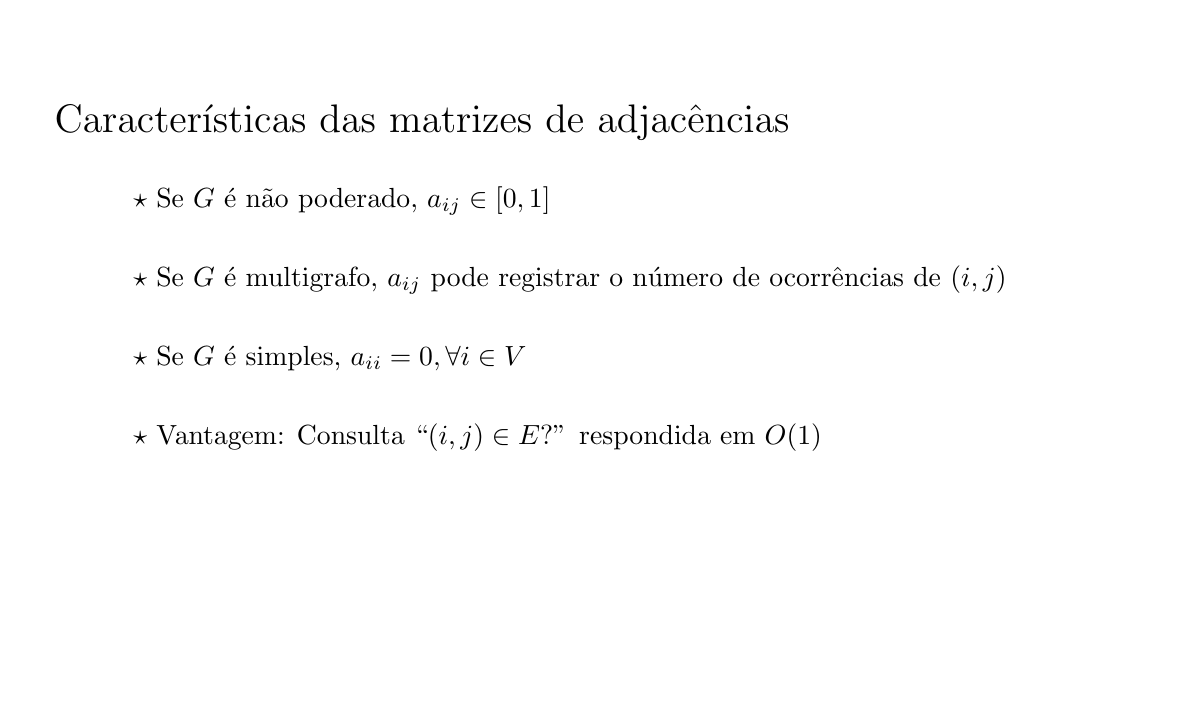
\begin{tikzpicture}
\node[draw,opacity=0] at (0, 0) {x};
\node[draw,opacity=0] at (14, 8) {x};
 \node[anchor=west] at (0, 7) { \Large \bbbold{Características das matrizes de adjacências} };
 \node[anchor=west] at (1, 6) { $\star$ \bbtext{Se $G$ é não poderado, $a_{ij} \in [0, 1]$ } };
 \node[anchor=west] at (1, 5) { $\star$ \bbtext{Se $G$ é multigrafo, $a_{ij}$ pode registrar o número de ocorrências de $(i, j)$ } };
 \node[anchor=west] at (1, 4) { $\star$ \bbtext{Se $G$ é simples, $a_{ii} = 0, \forall i\in V$} };
 \node[anchor=west] at (1, 3) { $\star$ \bbbold{Vantagem:} \bbtext{Consulta ``$(i, j)\in E$?'' respondida em $O(1)$} };
\end{tikzpicture}
\end{frame}

\begin{frame}[plain,t]
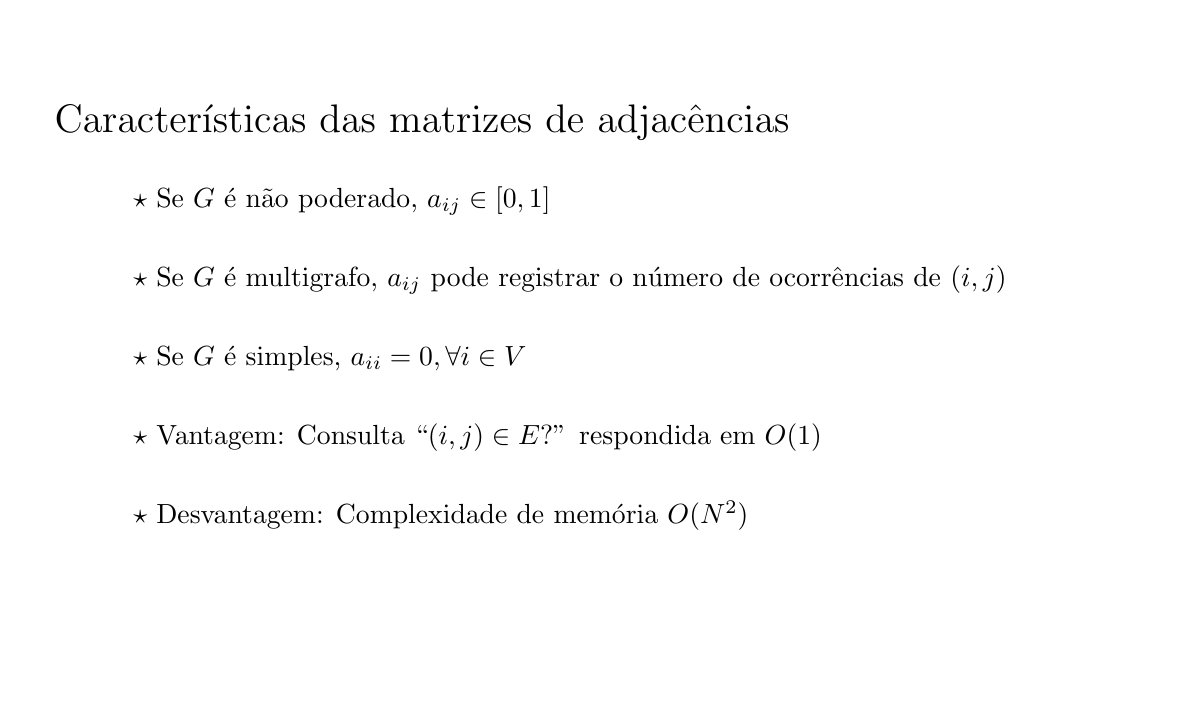
\begin{tikzpicture}
\node[draw,opacity=0] at (0, 0) {x};
\node[draw,opacity=0] at (14, 8) {x};
 \node[anchor=west] at (0, 7) { \Large \bbbold{Características das matrizes de adjacências} };
 \node[anchor=west] at (1, 6) { $\star$ \bbtext{Se $G$ é não poderado, $a_{ij} \in [0, 1]$ } };
 \node[anchor=west] at (1, 5) { $\star$ \bbtext{Se $G$ é multigrafo, $a_{ij}$ pode registrar o número de ocorrências de $(i, j)$ } };
 \node[anchor=west] at (1, 4) { $\star$ \bbtext{Se $G$ é simples, $a_{ii} = 0, \forall i\in V$} };
 \node[anchor=west] at (1, 3) { $\star$ \bbbold{Vantagem:} \bbtext{Consulta ``$(i, j)\in E$?'' respondida em $O(1)$} };
 \node[anchor=west] at (1, 2) { $\star$ \bbbold{Desvantagem:} \bbtext{Complexidade de memória $O(N^2)$} };
\end{tikzpicture}
\end{frame}

\begin{frame}[plain,t]
 \begin{center}\inputcode{cpp}{codes/matriz.cpp}\end{center}
\end{frame}

\begin{frame}[plain,t]
\begin{tikzpicture}
\node[draw,opacity=0] at (0, 0) {x};
\node[draw,opacity=0] at (14, 8) {x};
 \node[anchor=west] at (0, 6) { \Large \bbbold{Lista de adjacências} };
\end{tikzpicture}
\end{frame}

\begin{frame}[plain,t]
\begin{tikzpicture}
\node[draw,opacity=0] at (0, 0) {x};
\node[draw,opacity=0] at (14, 8) {x};
 \node[anchor=west] at (0, 6) { \Large \bbbold{Lista de adjacências} };
 \node[anchor=west] at (1, 5) { $\star$ \bbtext{A cada vértice $u$ é associada uma lista $l(u)$ } };
\end{tikzpicture}
\end{frame}

\begin{frame}[plain,t]
\begin{tikzpicture}
\node[draw,opacity=0] at (0, 0) {x};
\node[draw,opacity=0] at (14, 8) {x};
 \node[anchor=west] at (0, 6) { \Large \bbbold{Lista de adjacências} };
 \node[anchor=west] at (1, 5) { $\star$ \bbtext{A cada vértice $u$ é associada uma lista $l(u)$ } };
 \node[anchor=west] at (1, 4) { $\star$ \bbtext{Esta lista contém os vértices $v$ tais que $(u, v)\in E$} };
\end{tikzpicture}
\end{frame}

\begin{frame}[plain,t]
\begin{tikzpicture}
\node[draw,opacity=0] at (0, 0) {x};
\node[draw,opacity=0] at (14, 8) {x};
 \node[anchor=west] at (0, 6) { \Large \bbbold{Lista de adjacências} };
 \node[anchor=west] at (1, 5) { $\star$ \bbtext{A cada vértice $u$ é associada uma lista $l(u)$ } };
 \node[anchor=west] at (1, 4) { $\star$ \bbtext{Esta lista contém os vértices $v$ tais que $(u, v)\in E$} };
 \node[anchor=west] at (1, 3) { $\star$ \bbtext{Se $G$ é ponderado, então os elementos de $l(u)$ são pares $(v_i, w_i)$} };
\end{tikzpicture}
\end{frame}

\begin{frame}[plain,t]
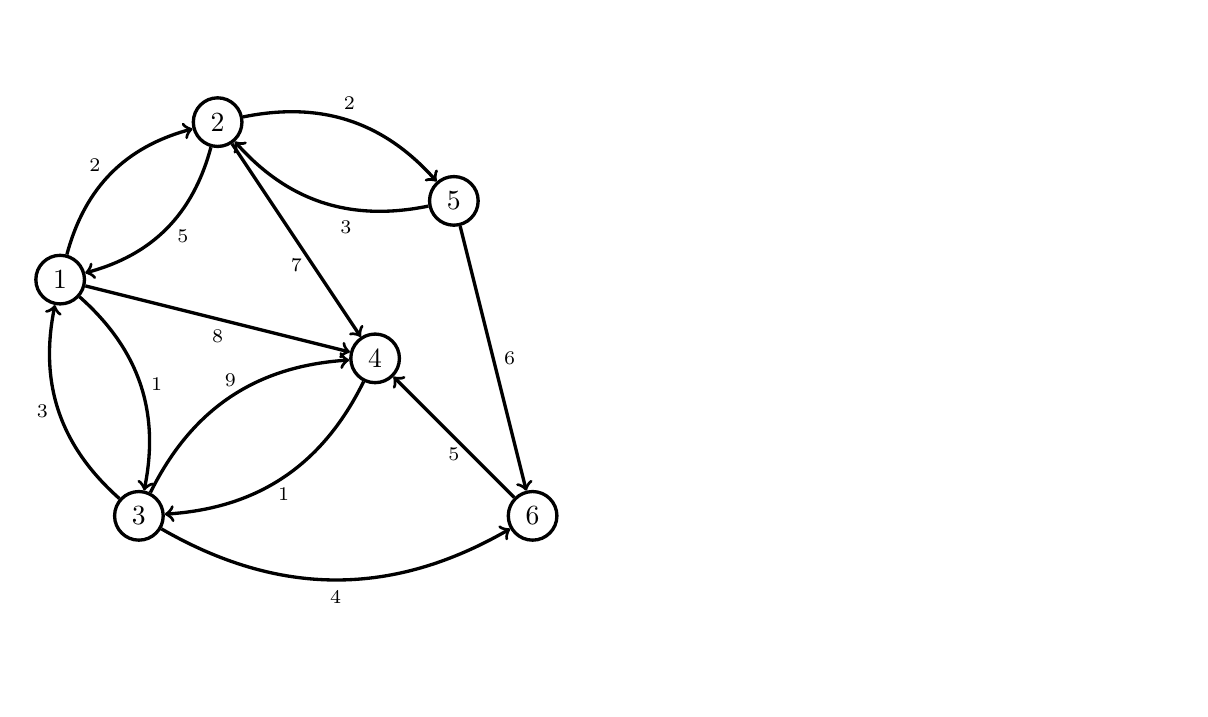
\begin{tikzpicture}
\node[draw,opacity=0] at (0, 0) {x};
\node[draw,opacity=0] at (14, 8) {x};
 \node[draw,circle,very thick] (A) at (0, 5) { \bbtext{1} };
 \node[draw,circle,very thick] (B) at (2, 7) { \bbtext{2} };
 \node[draw,circle,very thick] (C) at (1, 2) { \bbtext{3} };
 \node[draw,circle,very thick] (D) at (4, 4) { \bbtext{4} };
 \node[draw,circle,very thick] (E) at (5, 6) { \bbtext{5} };
 \node[draw,circle,very thick] (F) at (6, 2) { \bbtext{6} };
 \draw[->,very thick] (A) to [bend left] node[anchor=east,yshift=0.1cm] { \scriptsize $\bbinfo{2}$ } (B);
 \draw[->,very thick] (B) to [bend left] node[anchor=west,yshift=-0.1cm] { \scriptsize $\bbinfo{5}$ } (A);
 \draw[->,very thick] (A) to [bend left] node[anchor=west] { \scriptsize $\bbinfo{1}$ } (C);
 \draw[->,very thick] (C) to [bend left] node[anchor=east] { \scriptsize $\bbinfo{3}$ } (A);
 \draw[->,very thick] (D) to [bend left] node[anchor=north] { \scriptsize $\bbinfo{1}$ } (C);
 \draw[->,very thick] (C) to [bend left] node[anchor=south] { \scriptsize $\bbinfo{9}$ } (D);
 \draw[->,very thick] (B) to [bend left] node[anchor=south] { \scriptsize $\bbinfo{2}$ } (E);
 \draw[->,very thick] (E) to [bend left] node[anchor=north,xshift=0.3cm,yshift=-0.1cm] { \scriptsize $\bbinfo{3}$ } (B);
 \draw[->,very thick] (A) -- node[anchor=north] { \scriptsize $\bbinfo{8}$ } (D);
 \draw[->,very thick] (B) -- node[anchor=north,yshift=-0.1cm] { \scriptsize $\bbinfo{7}$ } (D);
 \draw[->,very thick] (C) to [bend right] node[anchor=north] { \scriptsize $\bbinfo{4}$ } (F);
 \draw[->,very thick] (F) -- node[anchor=north] { \scriptsize $\bbinfo{5}$ } (D);
 \draw[->,very thick] (E) -- node[anchor=west] { \scriptsize $\bbinfo{6}$ } (F);
\end{tikzpicture}
\end{frame}

\begin{frame}[plain,t]
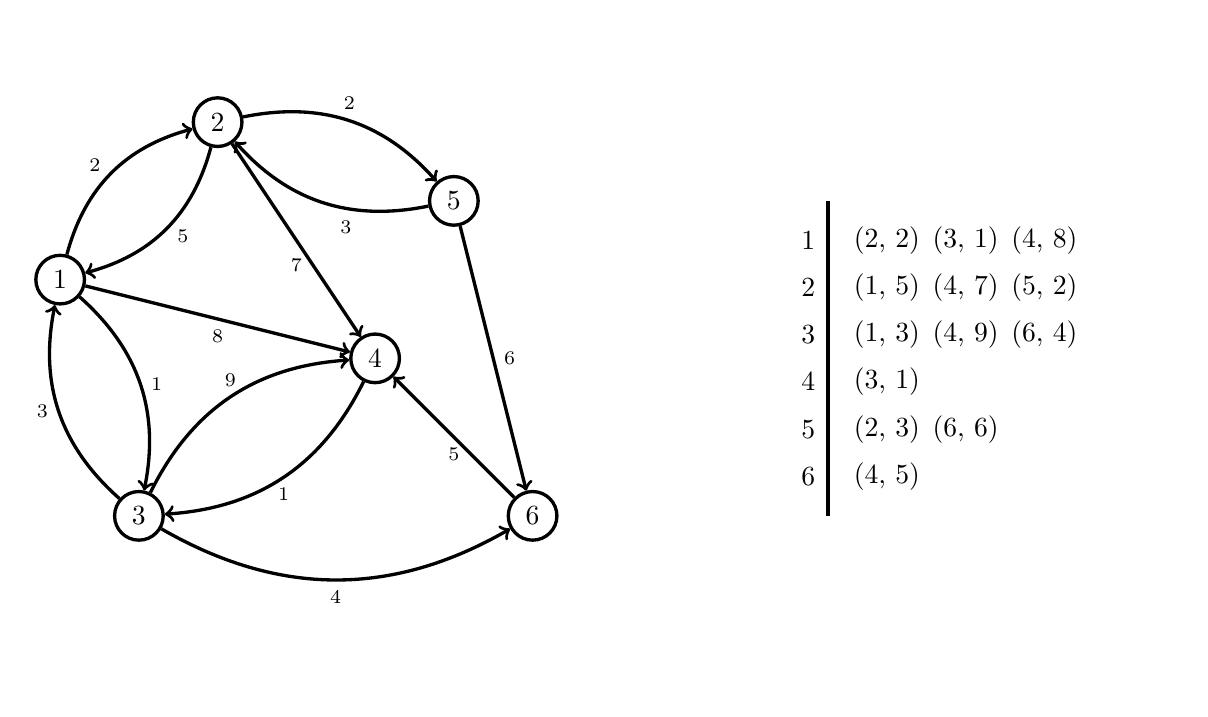
\begin{tikzpicture}
\node[draw,opacity=0] at (0, 0) {x};
\node[draw,opacity=0] at (14, 8) {x};
 \node[draw,circle,very thick] (A) at (0, 5) { \bbtext{1} };
 \node[draw,circle,very thick] (B) at (2, 7) { \bbtext{2} };
 \node[draw,circle,very thick] (C) at (1, 2) { \bbtext{3} };
 \node[draw,circle,very thick] (D) at (4, 4) { \bbtext{4} };
 \node[draw,circle,very thick] (E) at (5, 6) { \bbtext{5} };
 \node[draw,circle,very thick] (F) at (6, 2) { \bbtext{6} };
 \draw[->,very thick] (A) to [bend left] node[anchor=east,yshift=0.1cm] { \scriptsize $\bbinfo{2}$ } (B);
 \draw[->,very thick] (B) to [bend left] node[anchor=west,yshift=-0.1cm] { \scriptsize $\bbinfo{5}$ } (A);
 \draw[->,very thick] (A) to [bend left] node[anchor=west] { \scriptsize $\bbinfo{1}$ } (C);
 \draw[->,very thick] (C) to [bend left] node[anchor=east] { \scriptsize $\bbinfo{3}$ } (A);
 \draw[->,very thick] (D) to [bend left] node[anchor=north] { \scriptsize $\bbinfo{1}$ } (C);
 \draw[->,very thick] (C) to [bend left] node[anchor=south] { \scriptsize $\bbinfo{9}$ } (D);
 \draw[->,very thick] (B) to [bend left] node[anchor=south] { \scriptsize $\bbinfo{2}$ } (E);
 \draw[->,very thick] (E) to [bend left] node[anchor=north,xshift=0.3cm,yshift=-0.1cm] { \scriptsize $\bbinfo{3}$ } (B);
 \draw[->,very thick] (A) -- node[anchor=north] { \scriptsize $\bbinfo{8}$ } (D);
 \draw[->,very thick] (B) -- node[anchor=north,yshift=-0.1cm] { \scriptsize $\bbinfo{7}$ } (D);
 \draw[->,very thick] (C) to [bend right] node[anchor=north] { \scriptsize $\bbinfo{4}$ } (F);
 \draw[->,very thick] (F) -- node[anchor=north] { \scriptsize $\bbinfo{5}$ } (D);
 \draw[->,very thick] (E) -- node[anchor=west] { \scriptsize $\bbinfo{6}$ } (F);
 \draw[very thick] (9.75, 6) -- (9.75, 2);
 \node at (9.5, 5.5) { \bbtext{1} };
 \node at (10.5, 5.5) { \bbinfo{(2, 2)} };
 \node at (11.5, 5.5) { \bbinfo{(3, 1)} };
 \node at (12.5, 5.5) { \bbinfo{(4, 8)} };
 \node at (9.5, 4.9) { \bbtext{2} };
 \node at (10.5, 4.9) { \bbinfo{(1, 5)} };
 \node at (11.5, 4.9) { \bbinfo{(4, 7)} };
 \node at (12.5, 4.9) { \bbinfo{(5, 2)} };
 \node at (9.5, 4.3) { \bbtext{3} };
 \node at (10.5, 4.3) { \bbinfo{(1, 3)} };
 \node at (11.5, 4.3) { \bbinfo{(4, 9)} };
 \node at (12.5, 4.3) { \bbinfo{(6, 4)} };
 \node at (9.5, 3.7) { \bbtext{4} };
 \node at (10.5, 3.7) { \bbinfo{(3, 1)} };
 \node at (9.5, 3.1) { \bbtext{5} };
 \node at (10.5, 3.1) { \bbinfo{(2, 3)} };
 \node at (11.5, 3.1) { \bbinfo{(6, 6)} };
 \node at (9.5, 2.5) { \bbtext{6} };
 \node at (10.5, 2.5) { \bbinfo{(4, 5)} };
\end{tikzpicture}
\end{frame}

\begin{frame}[plain,t]
 \begin{center}\inputcode{cpp}{codes/listas.cpp}\end{center}
\end{frame}

\begin{frame}[plain,t]
\begin{tikzpicture}
\node[draw,opacity=0] at (0, 0) {x};
\node[draw,opacity=0] at (14, 8) {x};
 \node[anchor=west] at (0, 7) { \Large \bbbold{Características das listas de adjacências} };
\end{tikzpicture}
\end{frame}

\begin{frame}[plain,t]
\begin{tikzpicture}
\node[draw,opacity=0] at (0, 0) {x};
\node[draw,opacity=0] at (14, 8) {x};
 \node[anchor=west] at (0, 7) { \Large \bbbold{Características das listas de adjacências} };
 \node[anchor=west] at (1, 6) { $\star$ \bbtext{Possíveis listas em C++: \code{c}{list}, \code{c}{vector} ou \code{c}{forward_list}} };
\end{tikzpicture}
\end{frame}

\begin{frame}[plain,t]
\begin{tikzpicture}
\node[draw,opacity=0] at (0, 0) {x};
\node[draw,opacity=0] at (14, 8) {x};
 \node[anchor=west] at (0, 7) { \Large \bbbold{Características das listas de adjacências} };
 \node[anchor=west] at (1, 6) { $\star$ \bbtext{Possíveis listas em C++: \code{c}{list}, \code{c}{vector} ou \code{c}{forward_list}} };
 \node[anchor=west] at (1, 5) { $\star$ \bbtext{A escolha depende de como as arestas serão acessadas} };
\end{tikzpicture}
\end{frame}

\begin{frame}[plain,t]
\begin{tikzpicture}
\node[draw,opacity=0] at (0, 0) {x};
\node[draw,opacity=0] at (14, 8) {x};
 \node[anchor=west] at (0, 7) { \Large \bbbold{Características das listas de adjacências} };
 \node[anchor=west] at (1, 6) { $\star$ \bbtext{Possíveis listas em C++: \code{c}{list}, \code{c}{vector} ou \code{c}{forward_list}} };
 \node[anchor=west] at (1, 5) { $\star$ \bbtext{A escolha depende de como as arestas serão acessadas} };
 \node[anchor=west] at (1, 4) { $\star$ \bbtext{Complexidade de memória: $O(N + M)$, onde $M$ é o número de arestas} };
\end{tikzpicture}
\end{frame}

\begin{frame}[plain,t]
\begin{tikzpicture}
\node[draw,opacity=0] at (0, 0) {x};
\node[draw,opacity=0] at (14, 8) {x};
 \node[anchor=west] at (0, 7) { \Large \bbbold{Características das listas de adjacências} };
 \node[anchor=west] at (1, 6) { $\star$ \bbtext{Possíveis listas em C++: \code{c}{list}, \code{c}{vector} ou \code{c}{forward_list}} };
 \node[anchor=west] at (1, 5) { $\star$ \bbtext{A escolha depende de como as arestas serão acessadas} };
 \node[anchor=west] at (1, 4) { $\star$ \bbtext{Complexidade de memória: $O(N + M)$, onde $M$ é o número de arestas} };
 \node[anchor=west] at (1, 3) { $\star$ \bbtext{São adequadas para grafos esparsos} };
\end{tikzpicture}
\end{frame}

\begin{frame}[plain,t]
\begin{tikzpicture}
\node[draw,opacity=0] at (0, 0) {x};
\node[draw,opacity=0] at (14, 8) {x};
 \node[anchor=west] at (0, 7) { \Large \bbbold{Características das listas de adjacências} };
 \node[anchor=west] at (1, 6) { $\star$ \bbtext{Possíveis listas em C++: \code{c}{list}, \code{c}{vector} ou \code{c}{forward_list}} };
 \node[anchor=west] at (1, 5) { $\star$ \bbtext{A escolha depende de como as arestas serão acessadas} };
 \node[anchor=west] at (1, 4) { $\star$ \bbtext{Complexidade de memória: $O(N + M)$, onde $M$ é o número de arestas} };
 \node[anchor=west] at (1, 3) { $\star$ \bbtext{São adequadas para grafos esparsos} };
 \node[anchor=west] at (1, 2) { $\star$ \bbtext{Algoritmos clássicos utilizam esta representação} };
\end{tikzpicture}
\end{frame}

\begin{frame}[plain,t]
\begin{tikzpicture}
\node[draw,opacity=0] at (0, 0) {x};
\node[draw,opacity=0] at (14, 8) {x};
 \node[anchor=west] at (0, 6) { \Large \bbbold{Lista de arestas} };
\end{tikzpicture}
\end{frame}

\begin{frame}[plain,t]
\begin{tikzpicture}
\node[draw,opacity=0] at (0, 0) {x};
\node[draw,opacity=0] at (14, 8) {x};
 \node[anchor=west] at (0, 6) { \Large \bbbold{Lista de arestas} };
 \node[anchor=west] at (1, 5) { $\star$ \bbtext{O grafo $G$ é representado pelo conjunto de arestas $E$} };
\end{tikzpicture}
\end{frame}

\begin{frame}[plain,t]
\begin{tikzpicture}
\node[draw,opacity=0] at (0, 0) {x};
\node[draw,opacity=0] at (14, 8) {x};
 \node[anchor=west] at (0, 6) { \Large \bbbold{Lista de arestas} };
 \node[anchor=west] at (1, 5) { $\star$ \bbtext{O grafo $G$ é representado pelo conjunto de arestas $E$} };
 \node[anchor=west] at (1, 4) { $\star$ \bbtext{Cada aresta é representada pela tripla $(u, v, w)$} };
\end{tikzpicture}
\end{frame}

\begin{frame}[plain,t]
\begin{tikzpicture}
\node[draw,opacity=0] at (0, 0) {x};
\node[draw,opacity=0] at (14, 8) {x};
 \node[anchor=west] at (0, 6) { \Large \bbbold{Lista de arestas} };
 \node[anchor=west] at (1, 5) { $\star$ \bbtext{O grafo $G$ é representado pelo conjunto de arestas $E$} };
 \node[anchor=west] at (1, 4) { $\star$ \bbtext{Cada aresta é representada pela tripla $(u, v, w)$} };
 \node[anchor=west] at (1, 3) { $\star$ \bbtext{É possível deduzir $V$ a partir de $E$ se $G$ não tem vértices isolados} };
\end{tikzpicture}
\end{frame}

\begin{frame}[plain,t]
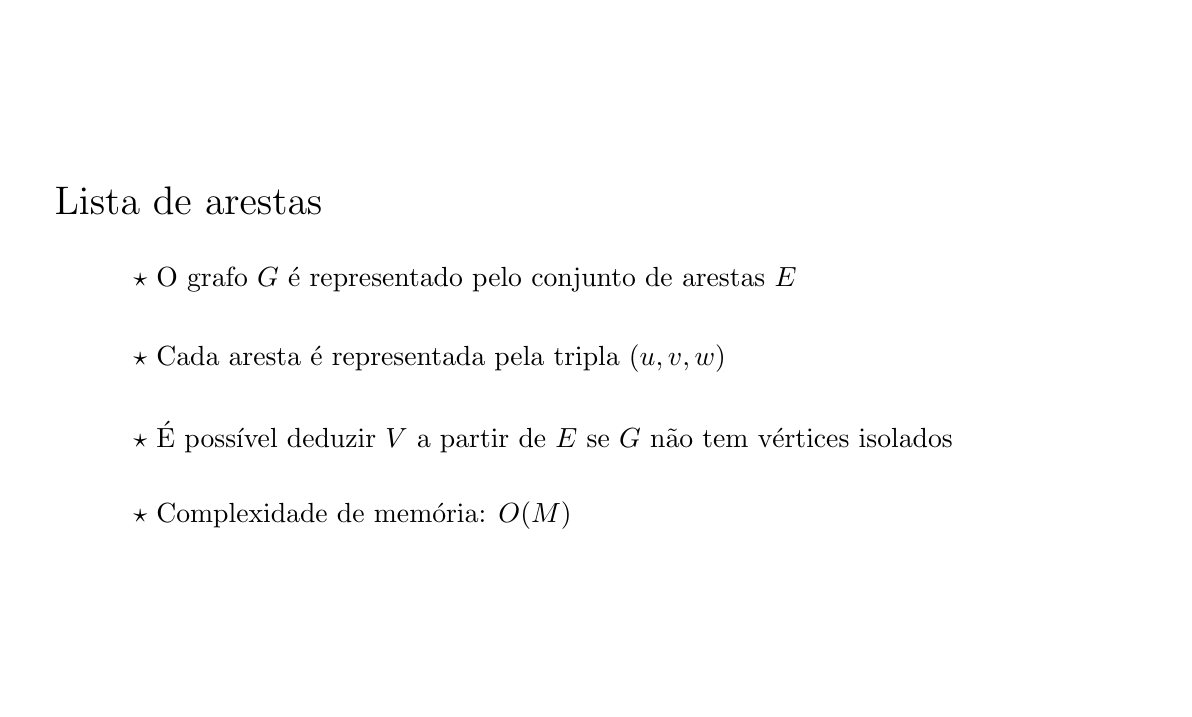
\begin{tikzpicture}
\node[draw,opacity=0] at (0, 0) {x};
\node[draw,opacity=0] at (14, 8) {x};
 \node[anchor=west] at (0, 6) { \Large \bbbold{Lista de arestas} };
 \node[anchor=west] at (1, 5) { $\star$ \bbtext{O grafo $G$ é representado pelo conjunto de arestas $E$} };
 \node[anchor=west] at (1, 4) { $\star$ \bbtext{Cada aresta é representada pela tripla $(u, v, w)$} };
 \node[anchor=west] at (1, 3) { $\star$ \bbtext{É possível deduzir $V$ a partir de $E$ se $G$ não tem vértices isolados} };
 \node[anchor=west] at (1, 2) { $\star$ \bbtext{Complexidade de memória: $O(M)$} };
\end{tikzpicture}
\end{frame}

\begin{frame}[plain,t]
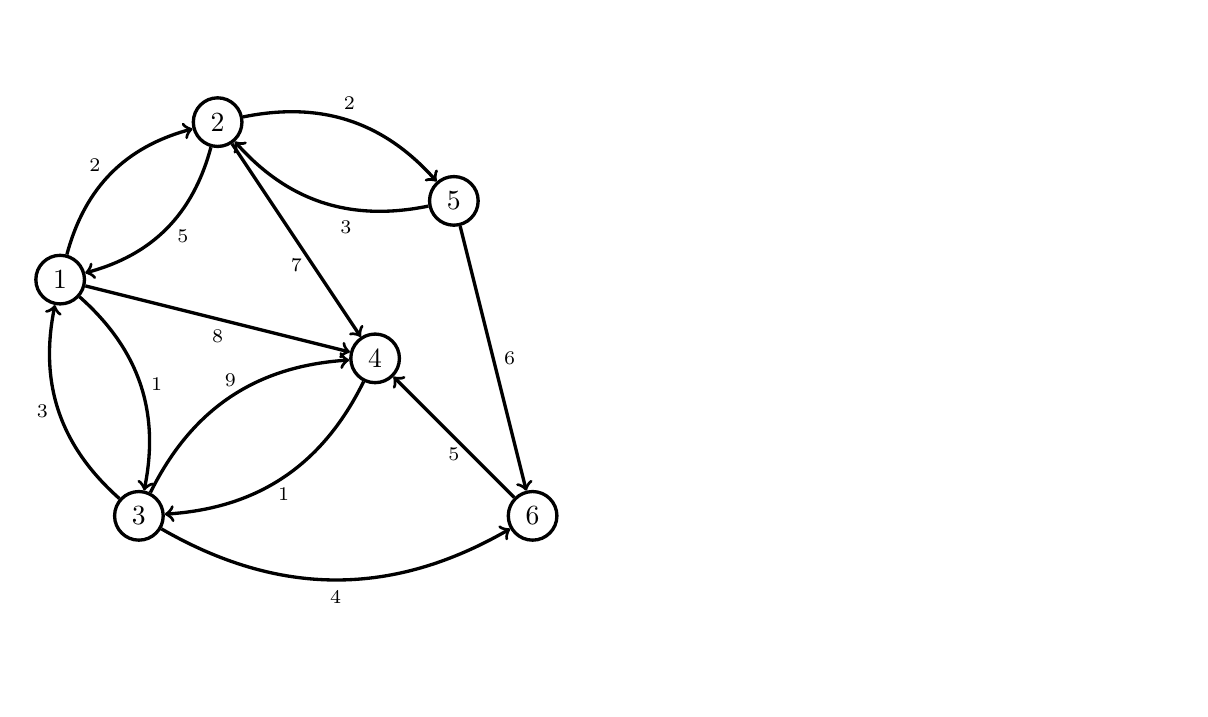
\begin{tikzpicture}
\node[draw,opacity=0] at (0, 0) {x};
\node[draw,opacity=0] at (14, 8) {x};
 \node[draw,circle,very thick] (A) at (0, 5) { \bbtext{1} };
 \node[draw,circle,very thick] (B) at (2, 7) { \bbtext{2} };
 \node[draw,circle,very thick] (C) at (1, 2) { \bbtext{3} };
 \node[draw,circle,very thick] (D) at (4, 4) { \bbtext{4} };
 \node[draw,circle,very thick] (E) at (5, 6) { \bbtext{5} };
 \node[draw,circle,very thick] (F) at (6, 2) { \bbtext{6} };
 \draw[->,very thick] (A) to [bend left] node[anchor=east,yshift=0.1cm] { \scriptsize $\bbinfo{2}$ } (B);
 \draw[->,very thick] (B) to [bend left] node[anchor=west,yshift=-0.1cm] { \scriptsize $\bbinfo{5}$ } (A);
 \draw[->,very thick] (A) to [bend left] node[anchor=west] { \scriptsize $\bbinfo{1}$ } (C);
 \draw[->,very thick] (C) to [bend left] node[anchor=east] { \scriptsize $\bbinfo{3}$ } (A);
 \draw[->,very thick] (D) to [bend left] node[anchor=north] { \scriptsize $\bbinfo{1}$ } (C);
 \draw[->,very thick] (C) to [bend left] node[anchor=south] { \scriptsize $\bbinfo{9}$ } (D);
 \draw[->,very thick] (B) to [bend left] node[anchor=south] { \scriptsize $\bbinfo{2}$ } (E);
 \draw[->,very thick] (E) to [bend left] node[anchor=north,xshift=0.3cm,yshift=-0.1cm] { \scriptsize $\bbinfo{3}$ } (B);
 \draw[->,very thick] (A) -- node[anchor=north] { \scriptsize $\bbinfo{8}$ } (D);
 \draw[->,very thick] (B) -- node[anchor=north,yshift=-0.1cm] { \scriptsize $\bbinfo{7}$ } (D);
 \draw[->,very thick] (C) to [bend right] node[anchor=north] { \scriptsize $\bbinfo{4}$ } (F);
 \draw[->,very thick] (F) -- node[anchor=north] { \scriptsize $\bbinfo{5}$ } (D);
 \draw[->,very thick] (E) -- node[anchor=west] { \scriptsize $\bbinfo{6}$ } (F);
\end{tikzpicture}
\end{frame}

\begin{frame}[plain,t]
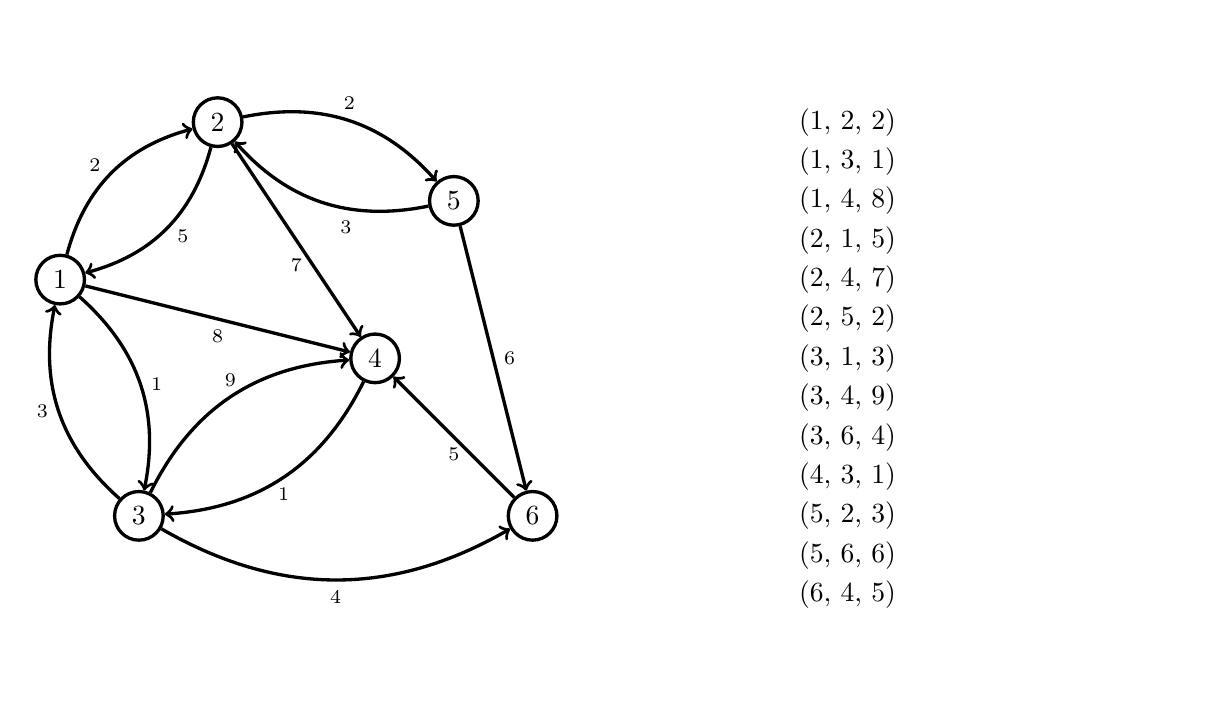
\begin{tikzpicture}
\node[draw,opacity=0] at (0, 0) {x};
\node[draw,opacity=0] at (14, 8) {x};
 \node[draw,circle,very thick] (A) at (0, 5) { \bbtext{1} };
 \node[draw,circle,very thick] (B) at (2, 7) { \bbtext{2} };
 \node[draw,circle,very thick] (C) at (1, 2) { \bbtext{3} };
 \node[draw,circle,very thick] (D) at (4, 4) { \bbtext{4} };
 \node[draw,circle,very thick] (E) at (5, 6) { \bbtext{5} };
 \node[draw,circle,very thick] (F) at (6, 2) { \bbtext{6} };
 \draw[->,very thick] (A) to [bend left] node[anchor=east,yshift=0.1cm] { \scriptsize $\bbinfo{2}$ } (B);
 \draw[->,very thick] (B) to [bend left] node[anchor=west,yshift=-0.1cm] { \scriptsize $\bbinfo{5}$ } (A);
 \draw[->,very thick] (A) to [bend left] node[anchor=west] { \scriptsize $\bbinfo{1}$ } (C);
 \draw[->,very thick] (C) to [bend left] node[anchor=east] { \scriptsize $\bbinfo{3}$ } (A);
 \draw[->,very thick] (D) to [bend left] node[anchor=north] { \scriptsize $\bbinfo{1}$ } (C);
 \draw[->,very thick] (C) to [bend left] node[anchor=south] { \scriptsize $\bbinfo{9}$ } (D);
 \draw[->,very thick] (B) to [bend left] node[anchor=south] { \scriptsize $\bbinfo{2}$ } (E);
 \draw[->,very thick] (E) to [bend left] node[anchor=north,xshift=0.3cm,yshift=-0.1cm] { \scriptsize $\bbinfo{3}$ } (B);
 \draw[->,very thick] (A) -- node[anchor=north] { \scriptsize $\bbinfo{8}$ } (D);
 \draw[->,very thick] (B) -- node[anchor=north,yshift=-0.1cm] { \scriptsize $\bbinfo{7}$ } (D);
 \draw[->,very thick] (C) to [bend right] node[anchor=north] { \scriptsize $\bbinfo{4}$ } (F);
 \draw[->,very thick] (F) -- node[anchor=north] { \scriptsize $\bbinfo{5}$ } (D);
 \draw[->,very thick] (E) -- node[anchor=west] { \scriptsize $\bbinfo{6}$ } (F);
 \node at (10, 7) { \bbinfo{(1, 2, 2)} };
 \node at (10, 6.5) { \bbinfo{(1, 3, 1)} };
 \node at (10, 6) { \bbinfo{(1, 4, 8)} };
 \node at (10, 5.5) { \bbinfo{(2, 1, 5)} };
 \node at (10, 5) { \bbinfo{(2, 4, 7)} };
 \node at (10, 4.5) { \bbinfo{(2, 5, 2)} };
 \node at (10, 4) { \bbinfo{(3, 1, 3)} };
 \node at (10, 3.5) { \bbinfo{(3, 4, 9)} };
 \node at (10, 3) { \bbinfo{(3, 6, 4)} };
 \node at (10, 2.5) { \bbinfo{(4, 3, 1)} };
 \node at (10, 2) { \bbinfo{(5, 2, 3)} };
 \node at (10, 1.5) { \bbinfo{(5, 6, 6)} };
 \node at (10, 1) { \bbinfo{(6, 4, 5)} };
\end{tikzpicture}
\end{frame}

\begin{frame}[plain,t]
 \begin{center}\inputcode{cpp}{codes/arestas.cpp}\end{center}
\end{frame}

\begin{frame}[plain,t]
\begin{tikzpicture}
\node[draw,opacity=0] at (0, 0) {x};
\node[draw,opacity=0] at (14, 8) {x};
 \node[anchor=west] at (0, 6) { \Large \bbbold{Representação implícita} };
\end{tikzpicture}
\end{frame}

\begin{frame}[plain,t]
\begin{tikzpicture}
\node[draw,opacity=0] at (0, 0) {x};
\node[draw,opacity=0] at (14, 8) {x};
 \node[anchor=west] at (0, 6) { \Large \bbbold{Representação implícita} };
 \node[anchor=west] at (1, 5) { $\star$ \bbtext{Os vértices e as arestas são definidas por relações} };
\end{tikzpicture}
\end{frame}

\begin{frame}[plain,t]
\begin{tikzpicture}
\node[draw,opacity=0] at (0, 0) {x};
\node[draw,opacity=0] at (14, 8) {x};
 \node[anchor=west] at (0, 6) { \Large \bbbold{Representação implícita} };
 \node[anchor=west] at (1, 5) { $\star$ \bbtext{Os vértices e as arestas são definidas por relações} };
 \node[anchor=west] at (1, 4) { $\star$ \bbtext{Adequada para grafos complexos ou com infinitos vértices e arestas} };
\end{tikzpicture}
\end{frame}

\begin{frame}[plain,t]
\begin{tikzpicture}
\node[draw,opacity=0] at (0, 0) {x};
\node[draw,opacity=0] at (14, 8) {x};
 \node[anchor=west] at (0, 6) { \Large \bbbold{Representação implícita} };
 \node[anchor=west] at (1, 5) { $\star$ \bbtext{Os vértices e as arestas são definidas por relações} };
 \node[anchor=west] at (1, 4) { $\star$ \bbtext{Adequada para grafos complexos ou com infinitos vértices e arestas} };
 \node[anchor=west] at (1, 3) { $\star$ \bbtext{Os elementos do grafo são identificados sob demanda} };
\end{tikzpicture}
\end{frame}

\begin{frame}[plain,t]
\begin{tikzpicture}
\node[draw,opacity=0] at (0, 0) {x};
\node[draw,opacity=0] at (14, 8) {x};
 \node[anchor=west] at (0, 7.5) { $G = G(V, E)$ };
 \node[anchor=west] at (0, 7) { $E = \{ (u, v)\in \mathbb{N}^2\ |\ u = kv, k\in \mathbb{N}\} $ };
\end{tikzpicture}
\end{frame}

\begin{frame}[plain,t]
\begin{tikzpicture}
\node[draw,opacity=0] at (0, 0) {x};
\node[draw,opacity=0] at (14, 8) {x};
 \node[anchor=west] at (0, 7.5) { $G = G(V, E)$ };
 \node[anchor=west] at (0, 7) { $E = \{ (u, v)\in \mathbb{N}^2\ |\ u = kv, k\in \mathbb{N}\} $ };
 \node[draw,circle,very thick] (A) at (3, 4) { \bbtext{1} };
 \node[draw,circle,very thick] (B) at (7, 5) { \bbtext{2} };
 \node[draw,circle,very thick] (C) at (7, 3) { \bbtext{3} };
 \node[draw,circle,very thick] (D) at (10, 6) { \bbtext{4} };
 \node[draw,circle,very thick] (E) at (10, 4) { \bbtext{5} };
 \node[draw,circle,very thick] (F) at (10, 2) { \bbtext{6} };
 \node[draw,circle,very thick] (G) at (13, 7) { \bbtext{7} };
 \node[draw,circle,very thick] (H) at (13, 5) { \bbtext{8} };
 \node[draw,circle,very thick] (I) at (13, 3) { \bbtext{9} };
 \node[draw,circle,very thick] (J) at (13, 1) { \bbtext{10} };
\end{tikzpicture}
\end{frame}

\begin{frame}[plain,t]
\begin{tikzpicture}
\node[draw,opacity=0] at (0, 0) {x};
\node[draw,opacity=0] at (14, 8) {x};
 \node[anchor=west] at (0, 7.5) { $G = G(V, E)$ };
 \node[anchor=west] at (0, 7) { $E = \{ (u, v)\in \mathbb{N}^2\ |\ u = kv, k\in \mathbb{N}\} $ };
 \node[draw,circle,very thick] (A) at (3, 4) { \bbtext{1} };
 \node[draw,circle,very thick] (B) at (7, 5) { \bbtext{2} };
 \node[draw,circle,very thick] (C) at (7, 3) { \bbtext{3} };
 \node[draw,circle,very thick] (D) at (10, 6) { \bbtext{4} };
 \node[draw,circle,very thick] (E) at (10, 4) { \bbtext{5} };
 \node[draw,circle,very thick] (F) at (10, 2) { \bbtext{6} };
 \node[draw,circle,very thick] (G) at (13, 7) { \bbtext{7} };
 \node[draw,circle,very thick] (H) at (13, 5) { \bbtext{8} };
 \node[draw,circle,very thick] (I) at (13, 3) { \bbtext{9} };
 \node[draw,circle,very thick] (J) at (13, 1) { \bbtext{10} };
 \draw[->,very thick] (B) to (A);
 \draw[->,very thick] (C) to (A);
\end{tikzpicture}
\end{frame}

\begin{frame}[plain,t]
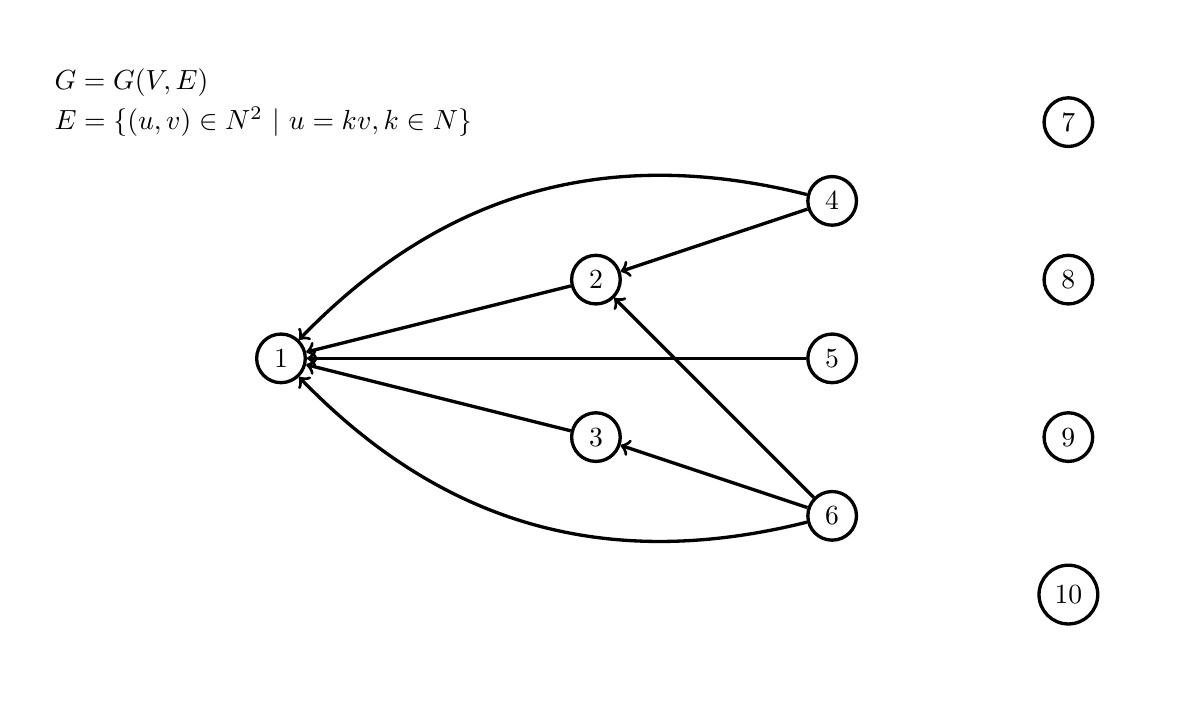
\begin{tikzpicture}
\node[draw,opacity=0] at (0, 0) {x};
\node[draw,opacity=0] at (14, 8) {x};
 \node[anchor=west] at (0, 7.5) { $G = G(V, E)$ };
 \node[anchor=west] at (0, 7) { $E = \{ (u, v)\in \mathbb{N}^2\ |\ u = kv, k\in \mathbb{N}\} $ };
 \node[draw,circle,very thick] (A) at (3, 4) { \bbtext{1} };
 \node[draw,circle,very thick] (B) at (7, 5) { \bbtext{2} };
 \node[draw,circle,very thick] (C) at (7, 3) { \bbtext{3} };
 \node[draw,circle,very thick] (D) at (10, 6) { \bbtext{4} };
 \node[draw,circle,very thick] (E) at (10, 4) { \bbtext{5} };
 \node[draw,circle,very thick] (F) at (10, 2) { \bbtext{6} };
 \node[draw,circle,very thick] (G) at (13, 7) { \bbtext{7} };
 \node[draw,circle,very thick] (H) at (13, 5) { \bbtext{8} };
 \node[draw,circle,very thick] (I) at (13, 3) { \bbtext{9} };
 \node[draw,circle,very thick] (J) at (13, 1) { \bbtext{10} };
 \draw[->,very thick] (B) to (A);
 \draw[->,very thick] (C) to (A);
 \draw[->,very thick] (D) [bend right] to (A);
 \draw[->,very thick] (D) to (B);
 \draw[->,very thick] (E) to (A);
 \draw[->,very thick] (F) [bend left] to (A);
 \draw[->,very thick] (F) to (B);
 \draw[->,very thick] (F) to (C);
\end{tikzpicture}
\end{frame}

\begin{frame}[plain,t]
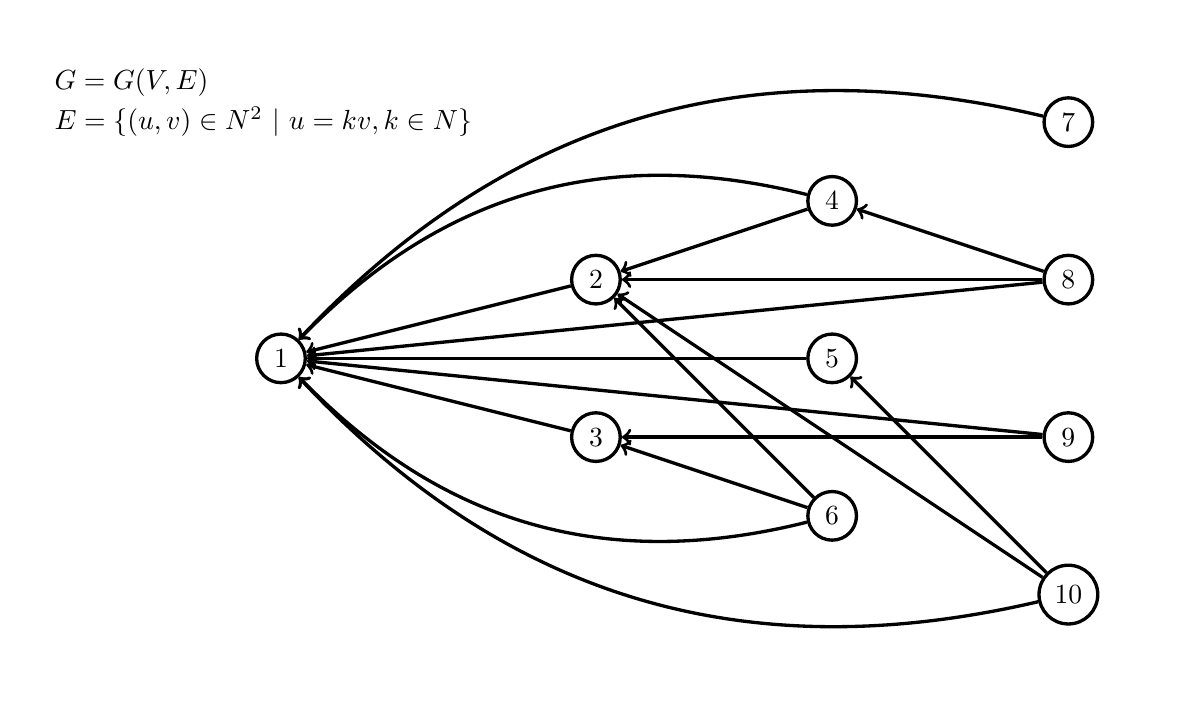
\begin{tikzpicture}
\node[draw,opacity=0] at (0, 0) {x};
\node[draw,opacity=0] at (14, 8) {x};
 \node[anchor=west] at (0, 7.5) { $G = G(V, E)$ };
 \node[anchor=west] at (0, 7) { $E = \{ (u, v)\in \mathbb{N}^2\ |\ u = kv, k\in \mathbb{N}\} $ };
 \node[draw,circle,very thick] (A) at (3, 4) { \bbtext{1} };
 \node[draw,circle,very thick] (B) at (7, 5) { \bbtext{2} };
 \node[draw,circle,very thick] (C) at (7, 3) { \bbtext{3} };
 \node[draw,circle,very thick] (D) at (10, 6) { \bbtext{4} };
 \node[draw,circle,very thick] (E) at (10, 4) { \bbtext{5} };
 \node[draw,circle,very thick] (F) at (10, 2) { \bbtext{6} };
 \node[draw,circle,very thick] (G) at (13, 7) { \bbtext{7} };
 \node[draw,circle,very thick] (H) at (13, 5) { \bbtext{8} };
 \node[draw,circle,very thick] (I) at (13, 3) { \bbtext{9} };
 \node[draw,circle,very thick] (J) at (13, 1) { \bbtext{10} };
 \draw[->,very thick] (B) to (A);
 \draw[->,very thick] (C) to (A);
 \draw[->,very thick] (D) [bend right] to (A);
 \draw[->,very thick] (D) to (B);
 \draw[->,very thick] (E) to (A);
 \draw[->,very thick] (F) [bend left] to (A);
 \draw[->,very thick] (F) to (B);
 \draw[->,very thick] (F) to (C);
 \draw[->,very thick] (G) [bend right] to (A);
 \draw[->,very thick] (H) to (A);
 \draw[->,very thick] (H) to (B);
 \draw[->,very thick] (H) to (D);
 \draw[->,very thick] (I) to (A);
 \draw[->,very thick] (I) to (C);
 \draw[->,very thick] (J) [bend left] to (A);
 \draw[->,very thick] (J) to (B);
 \draw[->,very thick] (J) to (E);
\end{tikzpicture}
\end{frame}

\begin{frame}[plain,t]
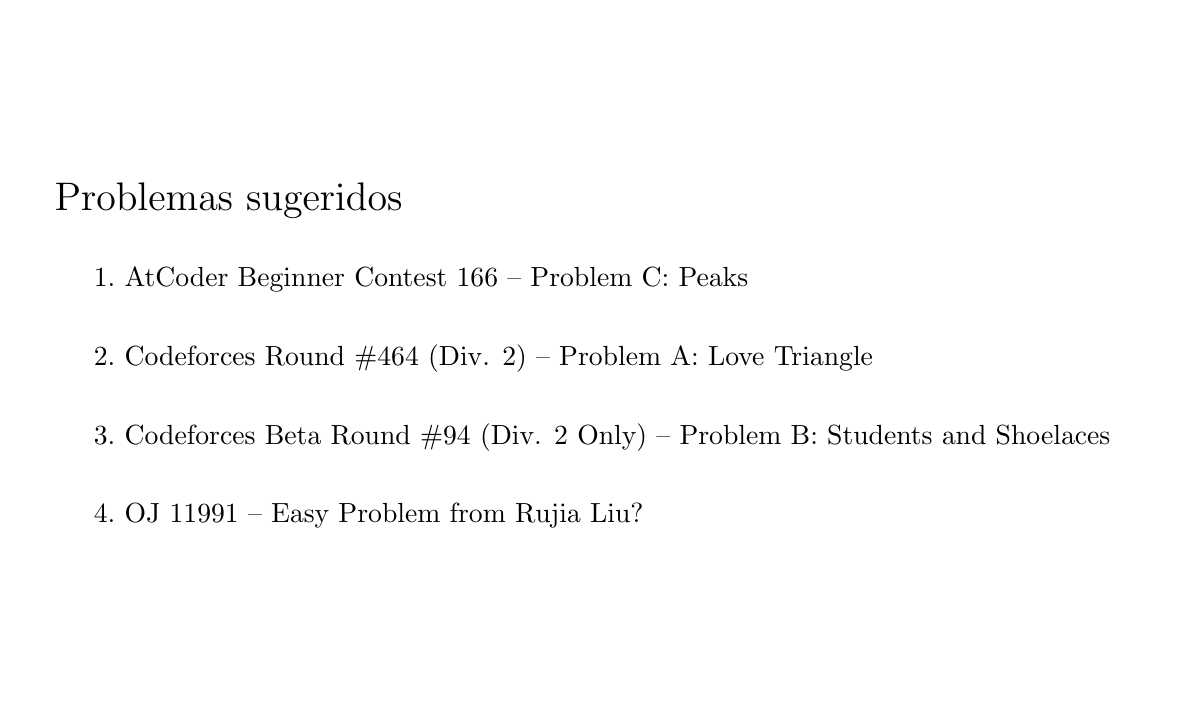
\begin{tikzpicture}
\node[draw,opacity=0] at (0, 0) {x};
\node[draw,opacity=0] at (14, 8) {x};
 \node[anchor=west] at (0, 6) { \Large \bbbold{Problemas sugeridos} };
 \node[anchor=west] at (0.5, 5) { $1.$ \bbtext{AtCoder Beginner Contest 166 -- Problem C: Peaks} };
 \node[anchor=west] at (0.5, 4) { $2.$ \bbtext{Codeforces Round \#464 (Div. 2) -- Problem A: Love Triangle} };
 \node[anchor=west] at (0.5, 3) { $3.$ \bbtext{Codeforces Beta Round \#94 (Div. 2 Only) -- Problem B: Students and Shoelaces} };
 \node[anchor=west] at (0.5, 2) { $4.$ \bbtext{OJ 11991 -- Easy Problem from Rujia Liu?} };
\end{tikzpicture}
\end{frame}

\begin{frame}[plain,t]

\begin{tikzpicture}
\node[draw,opacity=0] at (0, 0) {x};
\node[draw,opacity=0] at (14, 8) {x};
 \node[anchor=west] at (0, 6) { \Large \bbbold{Referências} };
 \node[anchor=west] at (1, 5) { $1.$ \bbbold{HALIM}, \bbtext{Felix}; \bbbold{HALIM}, \bbtext{Steve}. \bbenglish{Competitive Programming 3,} \bbtext{2010.} };
 \node[anchor=west] at (1, 4) { $2.$ \bbbold{LAAKSONEN}, \bbtext{Antti}. \bbenglish{Competitive Programmer's Handbook,} \bbtext{2018.} };
 \node[anchor=west] at (1, 3) { $3.$ \bbbold{SKIENA}, \bbtext{Steven}; \bbbold{REVILLA}, \bbtext{Miguel}. \bbenglish{Programming Challenges,} \bbtext{2003.} };
\end{tikzpicture}
\end{frame}

\end{document}
